\documentclass[a4paper,11pt]{article}
\usepackage{amsmath,amsthm,amsfonts,amssymb,amscd,amstext,vmargin,graphics,graphicx,tabularx,multicol} \usepackage[french]{babel}
\usepackage[utf8]{inputenc}  
\usepackage[T1]{fontenc} 
\usepackage[T1]{fontenc}
\usepackage{amsmath,amssymb}
\usepackage{pstricks-add,tikz,tkz-tab,variations}
\usepackage[autolanguage,np]{numprint} 

\setmarginsrb{1.5cm}{0.5cm}{1cm}{0.5cm}{0cm}{0cm}{0cm}{0cm} %Gauche, haut, droite, haut
\newcounter{numexo}
\newcommand{\exo}[1]{\stepcounter{numexo}\noindent{\bf Exercice~\thenumexo} : \marginpar{\hfill /#1}}
\reversemarginpar


\newcounter{enumtabi}
\newcounter{enumtaba}
\newcommand{\q}{\stepcounter{enumtabi} \theenumtabi.  }
\newcommand{\qa}{\stepcounter{enumtaba} (\alph{enumtaba}) }
\newcommand{\initq}{\setcounter{enumtabi}{0}}
\newcommand{\initqa}{\setcounter{enumtaba}{0}}

\newcommand{\be}{\begin{enumerate}}
\newcommand{\ee}{\end{enumerate}}
\newcommand{\bi}{\begin{itemize}}
\newcommand{\ei}{\end{itemize}}
\newcommand{\bp}{\begin{pspicture*}}
\newcommand{\ep}{\end{pspicture*}}
\newcommand{\bt}{\begin{tabular}}
\newcommand{\et}{\end{tabular}}
\renewcommand{\tabularxcolumn}[1]{>{\centering}m{#1}} %(colonne m{} centrée, au lieu de p par défault) 
\newcommand{\tnl}{\tabularnewline}

\newcommand{\trait}{\noindent \rule{\linewidth}{0.2mm}}
\newcommand{\hs}[1]{\hspace{#1}}
\newcommand{\vs}[1]{\vspace{#1}}

\newcommand{\N}{\mathbb{N}}
\newcommand{\Z}{\mathbb{Z}}
\newcommand{\R}{\mathbb{R}}
\newcommand{\C}{\mathbb{C}}
\newcommand{\Dcal}{\mathcal{D}}
\newcommand{\Ccal}{\mathcal{C}}
\newcommand{\mc}{\mathcal}

\newcommand{\vect}[1]{\overrightarrow{#1}}
\newcommand{\ds}{\displaystyle}
\newcommand{\eq}{\quad \Leftrightarrow \quad}
\newcommand{\vecti}{\vec{\imath}}
\newcommand{\vectj}{\vec{\jmath}}
\newcommand{\Oij}{(O;\vec{\imath}, \vec{\jmath})}
\newcommand{\OIJ}{(O;I,J)}

\newcommand{\bmul}[1]{\begin{multicols}{#1}}
\newcommand{\emul}{\end{multicols}}


\newcommand{\reponse}[1][1]{%
\multido{}{#1}{\makebox[\linewidth]{\rule[0pt]{0pt}{20pt}\dotfill}
}}

\newcommand{\titre}[5] 
% #1: titre #2: haut gauche #3: bas gauche #4: haut droite #5: bas droite
{
\noindent #2 \hfill #4 \\
#3 \hfill #5

\vspace{-1.6cm}

\begin{center}\rule{6cm}{0.5mm}\end{center}
\vspace{0.2cm}
\begin{center}{\large{\textbf{#1}}}\end{center}
\begin{center}\rule{6cm}{0.5mm}\end{center}
}



\begin{document}
\pagestyle{empty}
\titre{Contrôle : Calcul littéral, angles dans un triangle et fractions}{Nom :}{Prénom :}{Classe}{Date}


\exo{4}  Cours

\q	Énoncer la propriété concernant la mesure des angles d'un triangle isocèle.\\

\q Dans chacun des cas suivants, calculer la mesure du $3^{ème}$ angle, puis en déduire la nature exacte des triangles : \textbf{(pas de démonstration mais écrire les calculs)} \\

\qa Le triangle ABC est tel que :  $\widehat{BAC}$ = 42   et $\widehat{ACB} = 96$.

\qa Le triangle EFG est tel que :  $\widehat{FEG} = 60$   et   $\widehat{EFG}$ = 60.

\qa Le triangle IJK est tel que :   $\widehat{JIK}= 45$    et   $\widehat{JKI} = 90$\\


\exo{1,5}
Soit GTZ un triangle isocèle en T, tel que  : $\widehat{GTZ}$ = 112 .\\

\initq \q Faire un schéma à main levée puis calculer la mesure de  l'angle $\widehat{TZG}$. (Une démonstration est attendue) \\


\exo{4} Pour chacune des questions de cet exercice vous rédigerez des démonstrations en vous appuyant sur les propriétés vues en cours.

\bmul{2}
\initq
\q Calculer la mesure de l'angle $\widehat{UPO}$.

\includegraphics[scale=1]{rect.eps}

\columnbreak

\q Calculer la mesure de l'angle $\widehat{BED}$.

\includegraphics[scale=1]{complexe.eps} 
\emul


\exo{4} Pour chaque ligne, entourer la ou les propositions correctes.\\


\begin{tabular}{|c|c|c|c|c|}
\hline 
L'expression  & \multicolumn{4}{c|}{peut aussi s'écrire :} \\ 
\hline 
3 + 5 x 7 & (3 + 5) x 7 & 3 + (5 x 7) & 3 x 7 + 5 x 7 & (3 x 7) + (5 x 7) \\ 
\hline 
$4\times x + x^{2}$ & $4(x + x^{2})$ & $4 \times x^{3}$ & $5 \times x^{2}$ & $x(4 + x)$ \\ 
\hline 
2z + 3 + 4z + 5 & 6z + 8 & $14 \times z$ & 2z + 4z + 3 + 5 & (2 + 3 + 4 + 5)z \\ 
\hline 
$2a \times 3b$ & 23 x ab & 6ab & (2 + 3) x ab & 2 x 3 x a x b \\ 
\hline 
5x(1+7x) & $5x + 35x^{2}$ & 5x + 35x & $5x \times 1 + 5x \times 7x$ & $5x \times 1 \times 5x \times 7x$ \\ 
\hline 
\end{tabular} 

\vspace*{1cm}

\exo{1,5} Tester si l'expression $3x + 2 = 5x - 4$ est vraie pour x = 2 puis pour x = 3.\\


\exo{5,5}\initq \q Parmi les nombres suivants : 17 ; 233 ; 2115 ; 2523 ; 210 ; 468 ; 57

\noindent \initqa \qa Quels sont ceux qui sont divisibles par 2 ?\\
\qa Quels sont ceux qui sont divisibles par 3 ?\\
\qa Quels sont ceux qui sont divisibles par 5 ?\\
\qa Quels sont ceux qui sont divisibles par 9 ?\\

\q Quel est le critère de divisibilité par 4 ? Donner un exemple.\\

\q Simplifier les fractions suivantes le plus possible :
\bmul{2}

$\dfrac{54}{12}$

\columnbreak

$\dfrac{1260}{900}$

\emul


\end{document}
